%! TeX root = master.tex
% !TEX program = lualatex

\lecture{2}{2026-02-24}{Linear Regression (continuous insight)}{}

\subsection{1D linear regression}%
\label{sub:1D linear regression}
With 1D inputs, training a linear regressor aims to minimize 
\[ R\left(w^{\left(0\right)}, w^{\left(1\right)}\right) = \frac{1}{N}\sum_{i=1}^{N}d^2\left(\hat{y_i},y_i \right)=\frac{1}{N} \sum_{i = 1}^{N}\left(w^{\left(0\right)} + w^{\left(1\right)}x_i - y_i\right)^2 \]

Equivalently, we can write 
\[
  R\left(w\right) = \frac{1}{N}\sum_{i=1}^{N}\left(w^T x_i - y_i\right)^2 = \frac{1}{N}\sum_{i=1}^{N}\left(x_i^Tw - y_i\right)^2 
\]
where 
\[
x_i =\begin{pmatrix} 1 \\ x_i \end{pmatrix} \in \mathbb{R}^2 \qquad w = \begin{pmatrix} w^{(0)} \\ w^{(1)} \end{pmatrix} \in \mathbb{R}^2
\]
\subsection{Two input dimensions}%
\label{sub:two input dimensions}
\begin{wrapfigure}{r}{0.5\linewidth}
    %\centering
  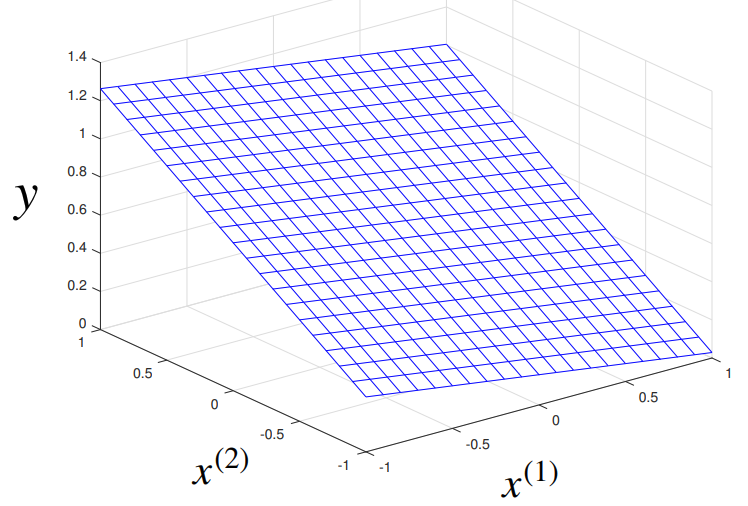
\includegraphics[width=\linewidth]{images/img_20260224_111948.png}
\end{wrapfigure}

Here instead of a line, we can define a plane. \\ 
Expressed 
\[
  y = w^{\left(0\right)} + w^{\left(1\right)}x^{\left(1\right)} + w^{\left(2\right)}x^{\left(2\right)} = w^T \begin{pmatrix} 1 \\ x^{\left(1\right)} \\ x^{\left(2\right)}\end{pmatrix}
\]

\subsection{Hyperplane}%
\label{sub:Hyperplane}
This can be generalized to higher dimensions. \\ 
In dimension D we can write 
\[
y = w^{\left(0\right)} + w^{\left(1\right)}x^{\left(1\right)} + w^{\left(2\right)}x^{\left(2\right)} + \ldots +  w^{\left(D\right)}x^{\left(D\right)}  = w^T \begin{pmatrix} 1 \\ x^{\left(1\right)} \\ x^{\left(2\right)} \\ \vdots \\x^{\left(D\right)} \end{pmatrix}
\]
Whatever the dimension, we can write 

\[
  y = w^Tx \quad x \in \mathbb{R}^{D+1}
\] , where the extra dimesion contains a 1 to account for $w^{\left(0\right)}$\\
  
Because the output remains 1D, we can still use the same least square loss function, and write training as 
\[
min_w \frac{1}{N}\sum_{i=1}^{N}d^2\left(\hat{y_i}, y_i\right) \iff min_w \frac{1}{N}\sum_{i=1}^{N}\left(x_i^Tw-y_i\right)^2  
\]
Solving this minimization problem involves computing its derivatives (derivation and gradient) w.r.t the model parameters (w). 

\subsection{Minimizing multivariate function}%
\label{sub:Minimizing multivariate function}
As in the 1D case (derivative = 0), to minimize a function, we seek the point \texbf{$w^*$} where the gradient where the gradient vanishes, i.e, 
\[
\nabla_wR(w^*) = 0
\]

\subsection{Solution of the linear regression}
With our least-square formulation, we seek to minimize
\[
  R(w) = \frac{1}{N}\sum_{i=1}^{N}(x_i^Tw - y_i)^2  
\]
This is a convex function of \textbf{w}, which means that we search for parameters \textbf{$w^*$} s.t
\[
 \nabla_w R(w^*) = 0 
\]   


Let us start by computing the gradient $\nabla_w R(w)$ \\

\textbf{Hint 1:} $R(w)$ is an average over the $N$ training samples
\begin{itemize}
  \item As the gradient of an average is the average of the gradients, you can focus on computing the gradient 
  \[
    \nabla_w(x_i^Tw - y_i)^2
  \]
\end{itemize}

\textbf{Hint 2:} Use the chain rule
\begin{itemize}
  \item The function $(x_i^Tw - y_i)^2$ has the form $f(g(w))$, with $f(g) = g^2$
  \item You can compute its gradient as $\frac{df(g)}{dg}\nabla_w g(w)$
\end{itemize}

\textbf{Hint 3:} To compute the gradient of g(w), you can make use of the following general vector derivative rule:
\begin{itemize}
  \item Given 2 vectors (a,b) in $\mathbb{R}^D$
    \[
    \nabla_b(a^Tb) = a
    \]
\end{itemize}

So with the chain rule:\\
\[
  \nabla_wR = \frac{1}{N}\sum_{i=1}^{N}\frac{d(x_i^Tw - y_i)^2}{d(x_i^Tw - y_i)} \cdot  \nabla_w(x_i^Tw - y_i) \\
= \frac{2}{N}\sum_{i=1}^{N}(x_i^Tw - y_i) \cdot x_i
\]

To obtain the solution, we search for $w^*$ s.t 
\[
  \nabla_wR(w^*) = \frac{2}{N}\sum_{i=1}^{N}x_i(x_i^Tw^* - y_i) = 0
\]
This means 
\[
  (\sum_{i=1}^{N}x_ix_i^T)w^* = \sum_{i=1}^{N}x_iy_i
\]
$(D+1) \times (D+1)$ matrix * $(D+1) \times 1$ vector = $(D+1) \times 1$ vector

Let us now group all ${x_i}$ and all ${y_i}$ in a matrix and a vector
\[
x = \begin{pmatrix} x_1^T \\ x_2^T \\ \vdots \\ x_N^T \end{pmatrix} = \begin{pmatrix} 1 & x_1^{(1)}& x_1^{(2)}& \dots & x_1^{(D)} \\ 1 & x_2^{(1)}& x_2^{(2)}& \dots & x_2^{(D)} \\ \vdots & \vdots & \vdots & \vdots & \vdots \\ 1 & x_N^{(1)}& x_N^{(2)}& \dots & x_N^{(D)}\end{pmatrix} \in \mathbb{R}^{N \times (D+1)}
\]
\[
  y = \begin{pmatrix} y_1 \\ y_2 \\ \vdots \\ y_N\end{pmatrix} \in \mathbb{R}^N
\]
Then we can re-write the solution as 
\[
  X^TXw^* = X^Ty
\]
This finally give us \[
  w^* = (X^TX)^{-1}X^Ty = X^\dagger y
\]
where $X^\dagger$ is known as the Moore-Penrose pseudo-inverse of X.

\subsection{Test time}
So now the predicted value $\hat{y_t}$ becomes 
\[
\hat{y_t} = \begin{pmatrix} 1\\x_t \end{pmatrix} ^T w^* = (w^*)^T\begin{pmatrix} 1\\ x_t\end{pmatrix}
\]

\section{Model evaluation}
Once an ML model is trained, one would typically understand how well it performs on unseen test data
\begin{itemize}
  \item At this stage, the parameters of the model are fixed
  \item Recall that the training and testing data must be separated!
\end{itemize}
During this evaluation, one compares the predictions of the model with the true annotations of the test data
\begin{itemize}
  \item In contrast to the training stage, the model parameters are not updated
  \item The evaluation metric may directly be the loss function, but may also differ from it
\end{itemize}

\subsection{Evaluation metrics for regression}
\textbf{Mean Squared Error (MSE)}: Same as the loss function but for $N_t$ test samples. 
\[
  MSE = \frac{1}{N_t}\sum_{i=1}^{N_t}(\hat{y_i} - y_i)^2 
\]
where $\hat{y_i}$ is the prediction for the test sample i and $y_i$ the corresponding ground-truth value\\

\textbf{Root Mean Squared Error (RMSE)}: Square-root of the MSE\\
\textbf{Mean Absolute Error (MAE)}
\[
  \frac{1}{N_t}\sum_{i=1}^{N_t}\left|\hat{y_i} - y_i\right|
\]
\textbf{Mean Absolute Percentage Error (MAPE)}
\[
  MAPE = \frac{1}{N_t}\sum_{i=1}^{N_t}\left|\frac{\hat{y_i} - y_i}{y_i}\right| 
\]

Example, UCI Wine Quality dataset, predict the quality of wine based on several attributes\\

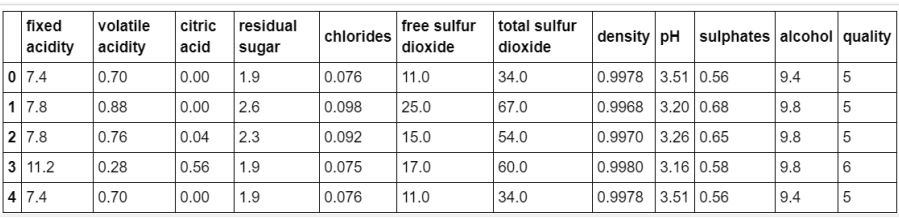
\includegraphics[width=\linewidth]{images/img_20260224_211627.png}
Here the final RMSE is 0.65 for the training data and 0.63 for the test data \\

\begin{wrapfigure}{r}{0.2\linewidth}
  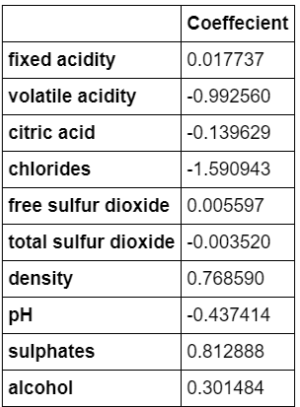
\includegraphics[width=\linewidth]{images/img_20260224_231831.png}
\end{wrapfigure}
One can the look at the coefficient values {$w^{(i)}$} to see the influence of each attribute\\
Warning: The magnitude of a coefficient will depend on the magnitude of the corresponding feature/attribute (A coefficient might be very small simply to compensate for the fact that the range of the feature is very large)

\subsection{Linear regression with multiple output dimensions}
Example of multiple output: human pose estimation
\subsection{Model}
The linear model has to be modified to output multiple values (not a vector w anymore because $w^Tx_i$ output a single value) \\
So we use a matrix \textbf{W} $\in \mathbb{R}^{(D+1)\times C}$ s.t 
\[
  \hat{y_i} = W^Tx_i = \begin{pmatrix} w_{(1)}^T \\ w_{(2)}^T \\ \vdots \\ w_{(C)}^T \end{pmatrix}x_i
\]
where each $w_{(j)}$ is a $(D+1)$-dimensional vector, used to predict one output dimension. \\
The multi-output linear regression is written
\[
  min_w \sum_{i=1}^{N}\left\|W^Tx_i - y_i\right\|^2
\]
where $\left\|a\right\| = \sqrt{\sum_{i=1}^{C}(a^{(j)})^2}$ indicates the norm of a vector (here a $\in \mathbb{R}^C$\\

To compute the gradient of this function, we make use of the following properties: \\
1. Norm and derivative:
\[
  \left\|a\right\|^2 = a^Ta
\]
and thus
\[
  \nabla_a \left\|a\right\|^2 = 2a
\]

2. Matrix derivative:
\[
  \nabla_B(a^TB) = a 
\]
Thus using the chain rule we obtain the gradient
\[
  \nabla_WR = 2 \sum_{i=1}^{N}x_i(x_i^TW - y_i^T) 
\]
setting it to zero means that
\[
  (\sum_{i=1}^{N}x_ix_i^T)W^* = \sum_{i=1}^{N}x_i y_i^T  
\]
$(D+1) \times (D+1)$ matrix * $(D+1) \times C$ matrix = $(D+1)\times C$ matrix \\
We can again group the inputs in a matrix \textbf{X} $\in \mathbb{R}^{N \times (D+1)}$, but the outputs now need to be grouped in a matrix (not a vector anymore), as 
\[
  Y = \begin{pmatrix} y_1^T \\ y_2^T \\ \vdots \\ y_N^T \end{pmatrix} = \begin{pmatrix} y_1^{(1)} &  y_1^{(2)} & \cdots & y_1^{(C)} \\ y_2^{(1)} &  y_2^{(2)} & \cdots & y_2^{(C)} \\ \vdots & \vdots & \vdots & \vdots \\ y_N^{(1)} &  y_N^{(2)} & \cdots & y_N^{(C)} \end{pmatrix} \in \mathbb{R}^{N \times C}
\]
Then, following the same strategy as before, we have
\[
W^* = (X^T X)^{-1}X^T Y = X^\dagger Y
\]

\section{Linear classification}
To predict one discrete label for a given sample e.g., binary classification or movies (like vs not), multi-class image recognition. \\
Classification can be tackle as a regression task (given a threshold we can classify the output in categories).\\
\begin{wrapfigure}{r}{0.4\linewidth}
  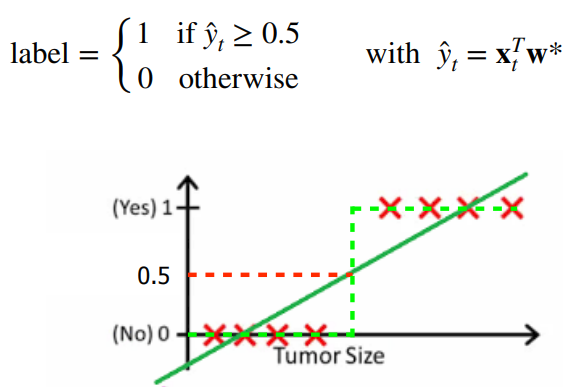
\includegraphics[width=\linewidth]{images/img_20260225_001349.png}
\end{wrapfigure}
E.g. Classify a tumor as benign vs malignant
\begin{itemize}
  \item 1D input (tumor size), 1D output (malignant/benign)
  \item Using a linear model, we can predict the label \\ $\hat{y} = w^{(0)} + w^{(1)}x$
\end{itemize}
To fit the linear model to training data, the same strategy as
for linear regression can be used:
\begin{itemize}
  \item Given N pairs {$(x_i, y_i)$} , we can use the least-square loss to write
    \[
      min_w \sum_{i=1}^{N}(x_i^Tw - y_i)^2  
    \]
\end{itemize}
So because the formulation is the same, the solution too
\[
  w^* = (X^TX)^{-1}X^Ty
\]
